% Figure blocks for the C&OR submission — generated with Experimental Result/plots (Figure.md).
% Widths are the design widths (90 / 140 / 190 mm); do not replace them with \linewidth.
% Captions follow Figure.md §4; lines marked "% CHANGED" deviate from the draft caption and say why.

% ---------------------------------------------------------------- FIG C1
\begin{figure}[t]
  \centering
  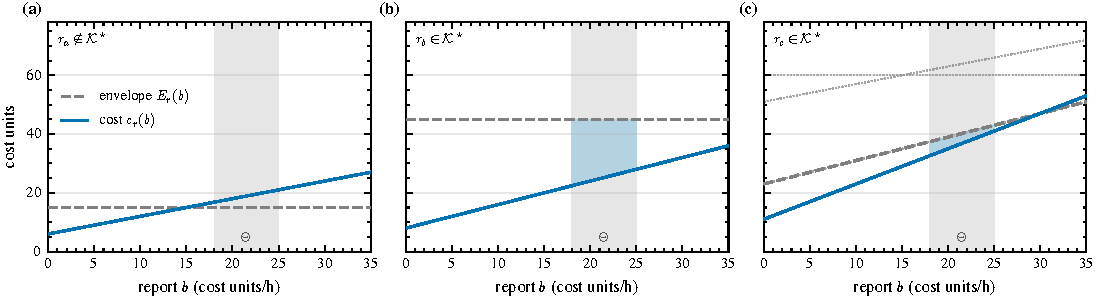
\includegraphics[width=190mm]{figures/fig_c1_frontier_intuition.pdf}
  \caption{Local margins in Example~11. Solid lines: reported cost $c_r(b)$; dashed: FD-completion
  envelope $E_r(b)$ (dotted in (c): its three affine branches); grey band: report domain
  $\Theta=[18,25]$. A route belongs to $\mathcal K^\star$ iff the envelope lies strictly above its cost
  somewhere in $\Theta$ (shaded). Route $r_a$ is deleted only because $\Theta$ excludes bids below 15;
  with unrestricted reports it would be retained (Remark~16).}
  \label{fig:frontier-intuition}
\end{figure}

% ---------------------------------------------------------------- FIG 1 — NOT PRODUCED (see MISSING.md)

% ---------------------------------------------------------------- FIG 2
\begin{figure}[t]
  \centering
  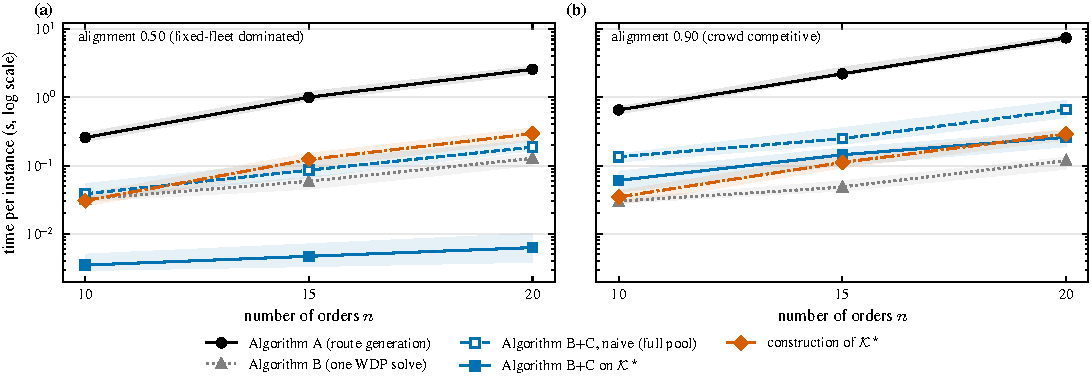
\includegraphics[width=190mm]{figures/fig02_runtime_breakdown.pdf}
  \caption{Median running time per component (log scale; bands: interquartile range) in the
  fixed-fleet-dominated regime (a) and the crowd-competitive regime (b), 100 instances per point.
  ``Algorithm B+C'' is one winner-determination solve plus one removal solve per winner; the WDP
  time of Algorithm B alone is taken from the bundling experiment on the same instances.
  The median time of exact VCG payment computation is at most 0.66\,s at $n=20$ (maximum over
  instances 1.15\,s); route generation dominates the pipeline.}
  % CHANGED: draft said "never exceed 0.66 s"; 0.66 s is the median, the maximum is 1.15 s.
  \label{fig:runtime-breakdown}
\end{figure}

% ---------------------------------------------------------------- FIG 3
\begin{figure}[t]
  \centering
  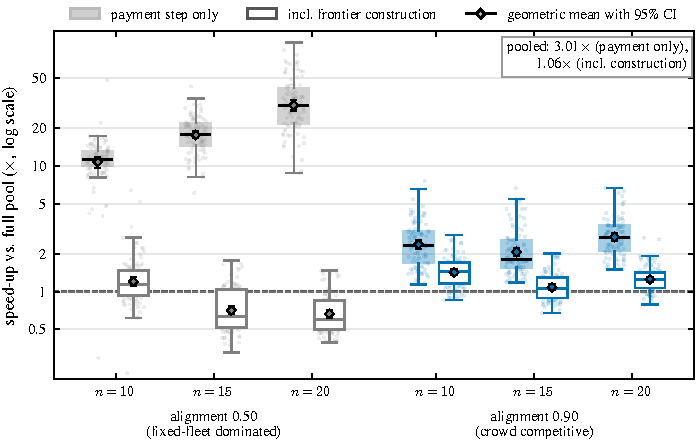
\includegraphics[width=140mm]{figures/fig03_payment_speedup.pdf}
  \caption{Speed-up of exact payment computation on the pruned pool $\mathcal K^\star$ relative to the
  full pool, per instance (log scale; boxes: IQR; diamonds: geometric mean with 95\% bootstrap CI).
  Filled boxes: payment step only; hollow boxes: including construction of the frontier. Pruning
  never changed a payment (maximum deviation $1.1\times10^{-13}$). The gain on the payment step is
  offset for a single auction by the cost of constructing the frontier in our implementation
  (pooled over 600 instances: $3.01\times$ for the payment step, $1.06\times$ including construction).}
  % CHANGED: added "geometric mean" (the mean is taken on the log scale shown).
  \label{fig:payment-speedup}
\end{figure}

% ---------------------------------------------------------------- FIG 4
\begin{figure}[t]
  \centering
  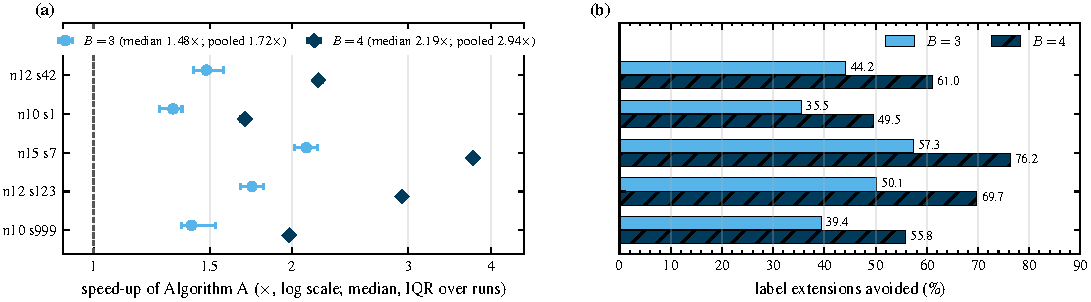
\includegraphics[width=190mm]{figures/fig04_label_rule.pdf}
  \caption{Effect of the FD-completion label rule on Algorithm A for the five experimental instances.
  (a) Speed-up per instance (median and IQR over 10 repeated runs; 20 for instance n10\,s999 at
  $B=3$); the legend gives the median over instances and the pooled total-time ratio. (b) Share of
  label extensions avoided. The rule leaves $\mathcal K^\star$ unchanged (Theorem~24) and never fired
  for occasional drivers.}
  \label{fig:label-rule}
\end{figure}

% ---------------------------------------------------------------- FIG 5
\begin{figure}[t]
  \centering
  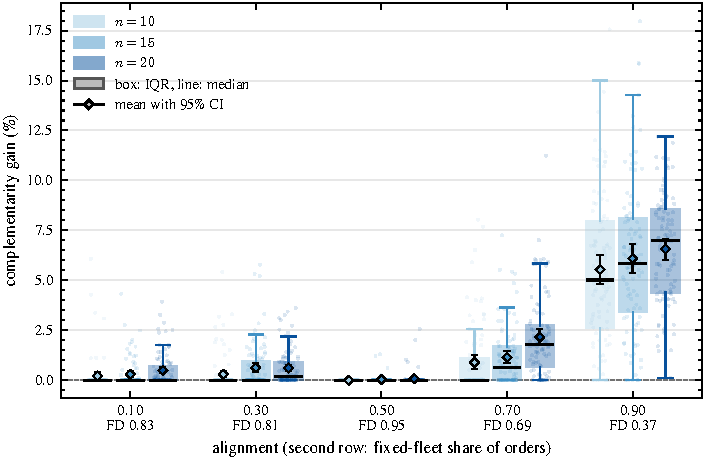
\includegraphics[width=140mm]{figures/fig05_rq1_complementarity.pdf}
  \caption{Complementarity gain of joint bidding over the better single-class procurement, per
  instance (100 instances per box). Second tick row: observed fixed-fleet share of orders. Boxes:
  IQR; diamonds: mean with 95\% bootstrap CI.}
  \label{fig:rq1-complementarity}
\end{figure}

% ---------------------------------------------------------------- FIG 5b (appendix)
\begin{figure}[t]
  \centering
  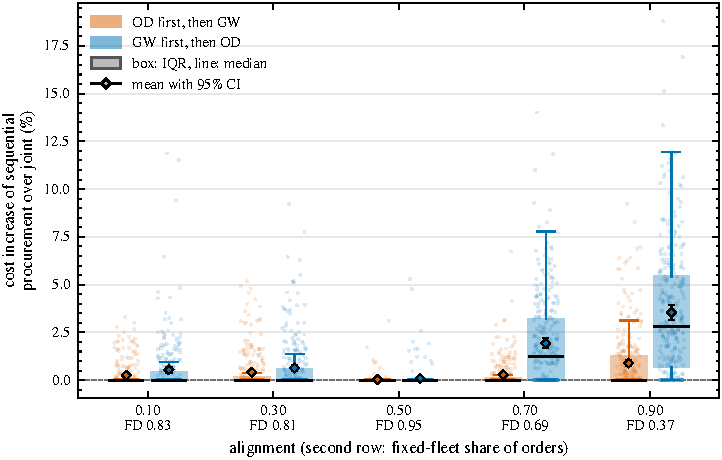
\includegraphics[width=140mm]{figures/fig05b_sequential.pdf}
  \caption{Cost increase of sequential procurement over joint bidding, per instance (300 instances
  per box). Consulting occasional drivers first recovers almost all of the joint value; consulting
  gigworkers first does not. Boxes: IQR; diamonds: mean with 95\% bootstrap CI.}
  \label{fig:rq1-sequential}
\end{figure}

% ---------------------------------------------------------------- FIG 6
\begin{figure}[t]
  \centering
  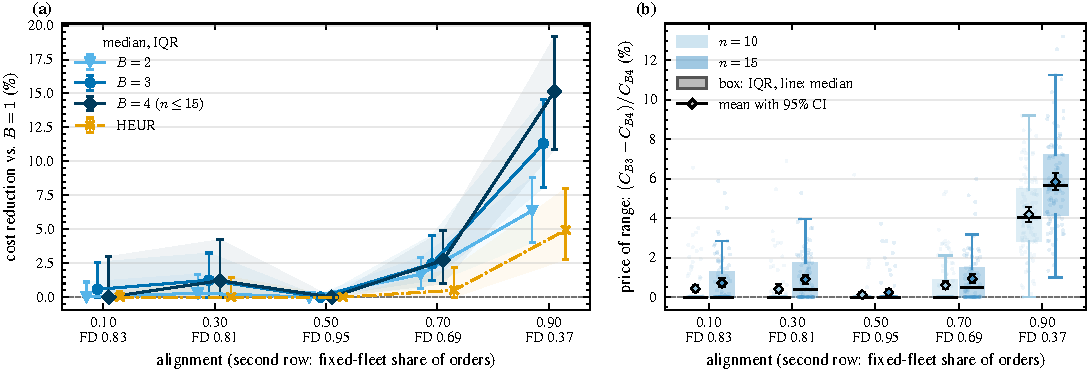
\includegraphics[width=190mm]{figures/fig06_rq2_bundling.pdf}
  \caption{(a) Cost reduction relative to single-order routes ($B=1$) for platform-generated bundles
  up to size 2, 3 and 4 and for a fixed bid-independent partition (HEUR); points: median, bars and
  bands: IQR; $B=4$ only for $n\le 15$. (b) Cost of restricting bundles to size 3 instead of 4.}
  \label{fig:rq2-bundling}
\end{figure}

% ---------------------------------------------------------------- FIG 7
\begin{figure}[t]
  \centering
  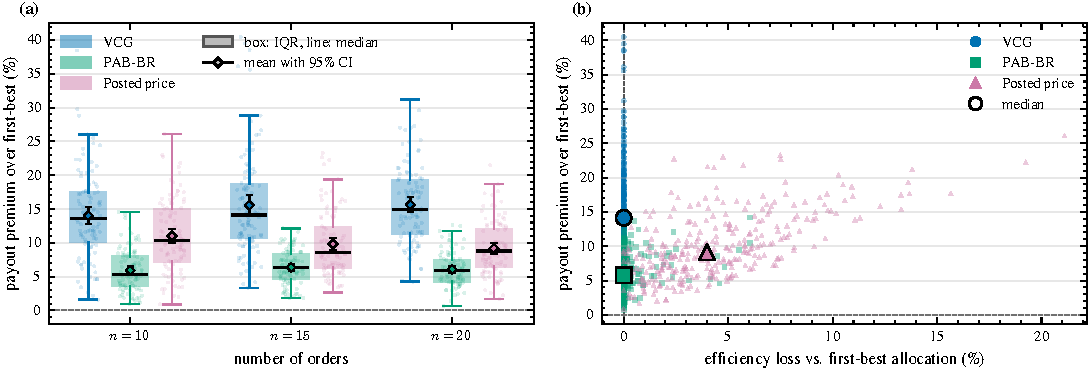
\includegraphics[width=190mm]{figures/fig07_rq3_mechanisms.pdf}
  \caption{Crowd-competitive regime (alignment 0.90, 300 instances). (a) Payout premium over the
  full-information benchmark. (b) Payout premium against efficiency loss per instance; large
  markers: medians. PAB-BR is a unilateral best-response benchmark within the bounded bid range,
  not an equilibrium. In the fixed-fleet-dominated regime all mechanisms coincide (not shown).}
  \label{fig:rq3-mechanisms}
\end{figure}

% ---------------------------------------------------------------- FIG 8
\begin{figure}[t]
  \centering
  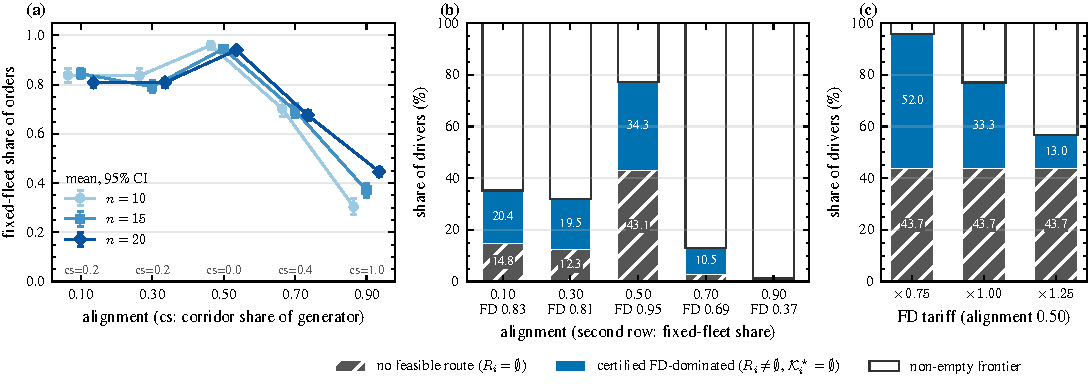
\includegraphics[width=190mm]{figures/fig08_regimes_certificate.pdf}
  \caption{(a) Share of orders served by the fixed fleet (mean over instances, 95\% CI; ``cs'':
  corridor share used by the generator); the share is not monotone in the nominal alignment level.
  (b--c) Drivers with no feasible route (hatched) and drivers whose feasible routes are all
  dominated by fixed-fleet completion over the entire report domain, i.e.\ certified before bidding
  by Theorem~4 (blue). The certified share falls monotonically with the fixed-fleet tariff, as
  predicted by Remark~14; the infeasible share does not depend on the tariff.}
  \label{fig:regimes-certificate}
\end{figure}

% ---------------------------------------------------------------- FIG 9
\begin{figure}[t]
  \centering
  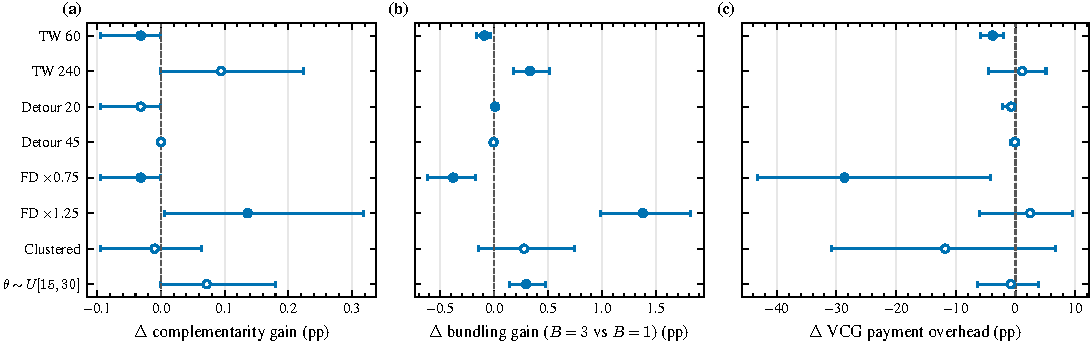
\includegraphics[width=190mm]{figures/fig09_rq5_forest.pdf}
  \caption{One-at-a-time robustness around the baseline (alignment 0.50, $n=15$): paired
  differences from the baseline (60 instances) in percentage points, with 95\% bootstrap CIs; filled
  markers: CI excludes zero. The baseline lies in the fixed-fleet-dominated regime, so most effects
  are close to zero; the fixed-fleet tariff is the governing parameter. Variant
  $\theta\sim U[15,30]$ changes the dispersion of true types; the VCG treatment of this study does
  not restrict reports to $\Theta$.}
  % CHANGED: added filled-marker key and the V8 sentence (Master Write-up §2.3, check 18.5).
  \label{fig:rq5-forest}
\end{figure}

% ---------------------------------------------------------------- FIG A1 — NOT PRODUCED (CHECK_FAILURES.md)

% ---------------------------------------------------------------- FIG A2
\begin{figure}[t]
  \centering
  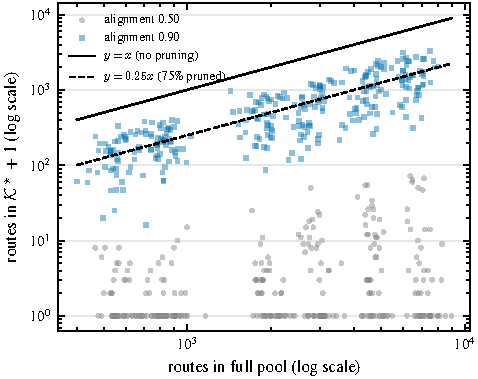
\includegraphics[width=90mm]{figures/figA2_pool_compression.pdf}
  \caption{Size of the local frontier against the full pool per instance (log--log; one is added to
  $|\mathcal K^\star|$ so that empty frontiers can be shown). Solid: no pruning; dashed: 75\% pruned.}
  \label{fig:pool-compression}
\end{figure}

% ---------------------------------------------------------------- FIG A3
\begin{figure}[t]
  \centering
  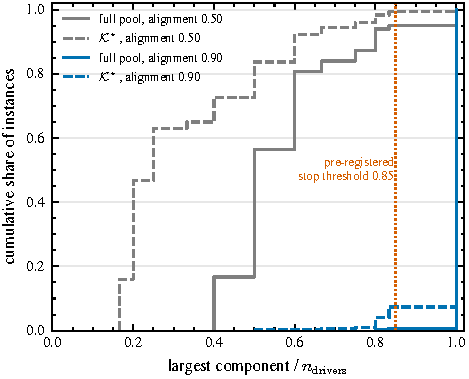
\includegraphics[width=90mm]{figures/figA3_t5_components.pdf}
  \caption{Empirical distribution of the largest conflict-graph component relative to the number of
  drivers, on the full pool and on $\mathcal K^\star$. On the crowd-competitive instances the conflict
  graph is almost always connected, so component decomposition yields little benefit. Dotted: the
  stopping threshold fixed before the run.}
  \label{fig:t5-components}
\end{figure}

% ---------------------------------------------------------------- FIG A4
\begin{figure}[t]
  \centering
  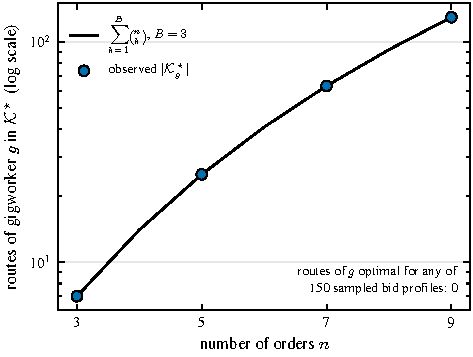
\includegraphics[width=90mm]{figures/figA4_synthetic_price_of_locality.pdf}
  \caption{Synthetic check of Theorem~10 ($B=3$): the frontier of gigworker $g$ keeps every route,
  $\sum_{k\le B}\binom nk$, although no route of $g$ is optimal for any of 150 sampled bid profiles.}
  \label{fig:synthetic-price-of-locality}
\end{figure}

% ---------------------------------------------------------------- FIG A5
\begin{figure}[t]
  \centering
  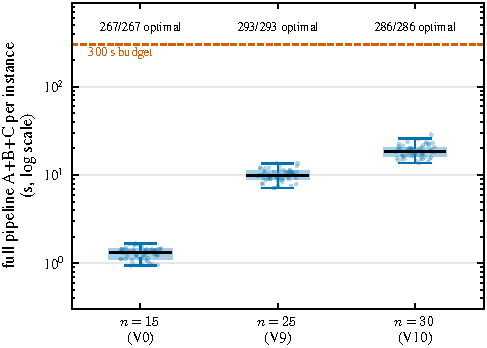
\includegraphics[width=90mm]{figures/figA5_pipeline_scaling.pdf}
  \caption{Running time of the full pipeline (Algorithms A, B and naive C) per instance (log
  scale). Dashed: 300\,s budget. Top: optimal solves over all solves. The $n=25$ and $n=30$ variants
  use one more gigworker and one more occasional driver than the $n=15$ baseline (supply
  $(3,3)$--$(4,4)$ instead of $(2,2)$--$(3,3)$).}
  \label{fig:pipeline-scaling}
\end{figure}

% ---------------------------------------------------------------- FIG A6, A7 — NOT PRODUCED (MISSING.md)
